\section{Auswertung}
\label{sec:Auswertung}
In diesem Abschnitt werden die Messdaten ausgewertet, um die Bragg Bedingung zu überprüfen, um das Emissionspektrum der Kupferröhre zu bestimmten und um die Absorptionsspektren von Brom, Gallium, Rubidium, Strontium und Zink zu bestimmen.
\subsection{Bragg}
Für die Überprüfung der Bragg Bedingung wurden die in \autoref{fig:bragg1} aufgelilsteten Daten verwendet.
\begin{figure}[H]
  \centering
  \includegraphics{daten/bragg.JPG}
  \caption{Bragg Daten}
  \label{fig:bragg1}
\end{figure}
In \autoref{fig:bragg2} wurden die pro Sekunde aufgenommenen Impulse in Abhänigkeit des Winkels dargestellt. Das gesuchte Maximum ist farblich markiert.
\begin{figure}[H]
  \centering
  \includegraphics{build/bragg.pdf}
  \caption{Bragg kreuze}
  \label{fig:bragg2}
\end{figure}
Das Maximum der Messdaten liegt bei $N=218 Imp/s$ mit dem Winkel $\theta=28.2°$. Der theoretische Glanzwinkel für die Anordnung mit dem LiF-Kristall lässt sich nach \autoref{eqn:braggsche-bedingung} berechnen.
\subsection{Emissionsspektrum}
\begin{figure}[H]
  \centering
  \includegraphics{build/spektrum.pdf}
  \caption{Spektrum}
  \label{fig:spektrum}
\end{figure}
\subsection{Abschirmung}

\begin{figure}[H]
  \centering
  \includegraphics{build/Brom.pdf}
  \caption{Brom}
  \label{fig:Brom}
\end{figure}

\begin{figure}[H]
  \centering
  \includegraphics{build/Gallium.pdf}
  \caption{Gallium}
  \label{fig:Gallium}
\end{figure}

\begin{figure}[H]
  \centering
  \includegraphics{build/Rubidium.pdf}
  \caption{Rubidium}
  \label{fig:Rubidium}
\end{figure}

\begin{figure}[H]
  \centering
  \includegraphics{build/Strontium.pdf}
  \caption{Strontium}
  \label{fig:Strontium}
\end{figure}

\begin{figure}[H]
  \centering
  \includegraphics{build/Zink.pdf}
  \caption{Zink}
  \label{fig:Zink}
\end{figure}